\chapter{Korosi dan Proteksi}\label{ch:b2:corrosion}

Teteskan setetes air garam pada sepotong baja yang bersih. Setelah sehari,
logam itu berlubang-lubang di tengah tetesan, sedangkan karatnya terbentuk
sebagai cincin di dekat tepinya, tempat oksigen dari udara larut. Besi
larut di tempat oksigennya paling sedikit, dan oksigen direduksi di tempat
oksigennya paling banyak: tetesan itu adalah sebuah sel yang tidak dibuat
siapa pun, yang terhubung singkat melalui logam itu sendiri. Bab ini
membaca korosi pada \omterm{def:b2:current-potential-curves:ie-curve}{kurva arus--potensial}, menjelaskan mengapa lembaran
galvanis yang tergores tidak berkarat sedangkan kaleng timah yang tergores
berkarat, dan merancang proteksi sebuah pipa yang ditanam di dalam tanah.

\begin{recall}
Jilid Tahun 1: diagram E--pH logam-logam dan daerah imunitas, korosi, dan
\omterm{def:b2:corrosion:passivation}{pasivasinya} (``apakah sebuah lapisan melindungi adalah persoalan
kinetika''). \Cref{ch:b2:current-potential-curves}: \omterm{def:b2:current-potential-curves:ie-curve}{kurva arus--potensial},
\omterm{def:b2:current-potential-curves:limiting-current}{arus pembatas}. \Cref{ch:b2:batteries-electrolysis}: \omterm{def:b2:batteries-electrolysis:mixed-potential}{potensial campuran}.
Jilid sekolah: korosi, karat, galvanisasi.
\end{recall}

\begin{omfigure}
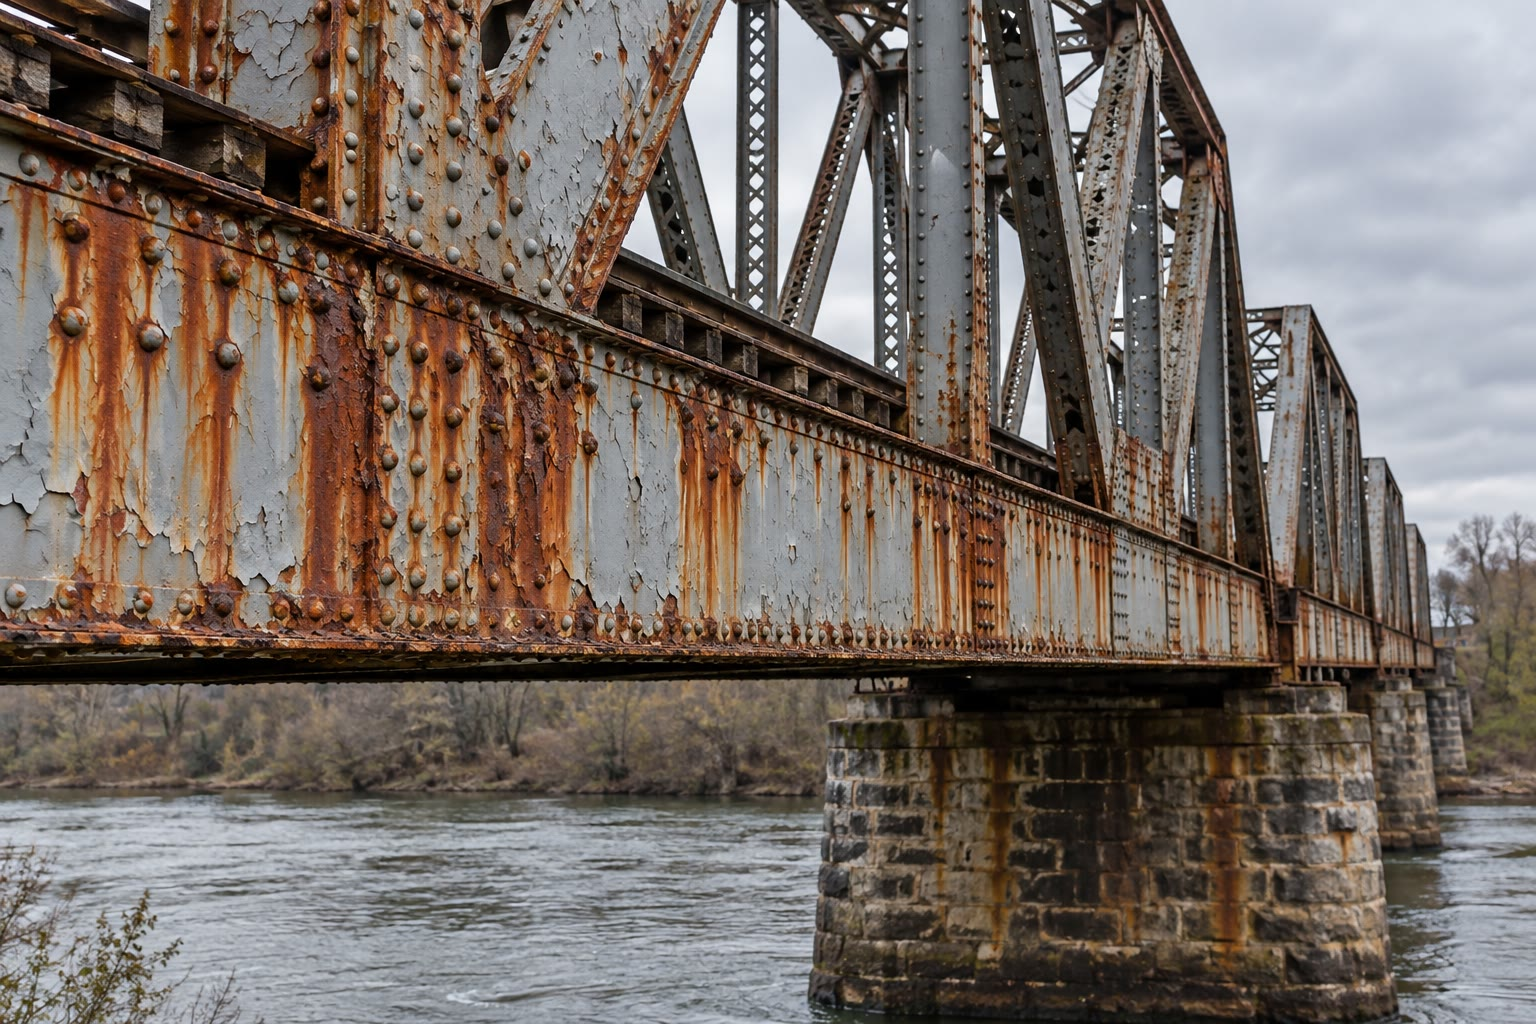
\includegraphics[width=0.62\linewidth]{images/book3/ai/b2-12-rusty-bridge.jpg}

{\small Sebuah jembatan kereta api tua yang dikeling. Garis-garis karat
mengalir turun dari paku-paku keling dan sambungan, tempat air dan oksigen
paling lama tertahan dan catnya paling dahulu rusak.}
\end{omfigure}

\section{Korosi basah sebagai sel yang terhubung singkat}

Dalam air yang mengandung oksigen terlarut, besi dioksidasi,
\ce{Fe -> Fe^2+ + 2e-}, dan elektron-elektronnya diambil pada potongan
logam yang sama oleh reduksi dioksigen, \ce{O2 + 2H2O + 4e- -> 4OH-} (dalam
asam, juga oleh \ce{2H+ + 2e- -> H2}). Ion-ion besi(II) dan ion-ion
hidroksida bertemu di dalam air, dan oksidasi lebih lanjut oleh udara
mengubah endapannya menjadi karat, sebuah besi(III) oksida terhidrat.

\begin{definition}[Korosi seragam]\label{def:b2:corrosion:uniform}
Yang disebut \emph{korosi seragam}\index{korosi seragam} adalah korosi
sebuah logam yang oksidasinya dan reduksi oksidatornya berlangsung di
situs-situs yang tersebar merata di permukaannya. Yang disebut
\emph{potensial korosi}\index{potensial korosi} adalah \omterm{def:b2:batteries-electrolysis:mixed-potential}{potensial campuran}
yang lalu diambil logam itu, dan \emph{arus korosi}\index{arus korosi}
adalah \omterm{def:b2:current-potential-curves:ie-curve}{arus anodik} oksidasi logam pada potensial itu.
\end{definition}

\begin{omfigure}
\begin{tikzpicture}
\begin{axis}[omie, width=0.82\linewidth, height=5.6cm, xmin=-1.1, xmax=0.5,
  ymin=-1.6, ymax=1.6, xlabel={$E$}, ylabel={$i$}, clip=true, clip mode=individual,
  axis y line=left]
\addplot[omanodic] table[x=E, y=i] {figdata/out/bachelor-2-ie-curves-i-Fe.dat};
\addplot[omcathodic] table[x=E, y=i] {figdata/out/bachelor-2-ie-curves-i-O2.dat};
\addplot[omcathodic, densely dashed] table[x=E, y=i, y expr=-\thisrow{i}] {figdata/out/bachelor-2-ie-curves-i-O2.dat};
\draw[densely dotted] (axis cs:-0.394,-1.0) -- (axis cs:-0.394,1.0);
\fill (axis cs:-0.394,1.0) circle (1.4pt);
\node[font=\scriptsize, anchor=south east] at (axis cs:-0.40,1.02) {$i_{\text{kor}}$};
\node[font=\scriptsize, anchor=north west] at (axis cs:-0.39,-0.03) {$E_{\text{kor}}$};
\node[font=\scriptsize, omThm, anchor=west] at (axis cs:-0.35,1.4) {\ce{Fe} $\to$ \ce{Fe^2+}};
\node[font=\scriptsize, omDef, anchor=north west] at (axis cs:-0.75,-1.05) {\ce{O2} $\to$ \ce{OH-}, plato difusi};
\end{axis}
\end{tikzpicture}

{\small Diagram Evans besi dalam air netral yang beraerasi (kurva model).
Kurva katodik dioksigen juga digambar terpantul ke atas (putus-putus):
\omterm{def:b2:corrosion:uniform}{potensial korosi} terletak di tempat kurva itu bertemu dengan kurva anodik
besi. Karena reduksi dioksigen telah mencapai plato difusinya di sana, \omterm{def:b2:corrosion:uniform}{arus
korosi} sama dengan \omterm{def:b2:current-potential-curves:limiting-current}{arus pembatas} oksigen: mengaduk atau mengaerasi air
membuat besi terkorosi lebih cepat.}
\end{omfigure}

\begin{proposition}[Laju korosi]\label{prop:b2:corrosion:rate}
Logam bermassa molar $M$ dan bermassa jenis $\rho$, yang dioksidasi dengan
$n$ elektron per atom di bawah rapat \omterm{def:b2:corrosion:uniform}{arus korosi} $j_{\text{kor}}$ (arus
per satuan luas), kehilangan per satuan luas per satuan waktu massa
$j_{\text{kor}}M/(nF)$, yaitu ketebalan
\[
  \frac{de}{dt} = \frac{j_{\text{kor}}\,M}{nF\rho} .
\]
\end{proposition}

\begin{proof}
Menurut \cref{prop:b2:current-potential-curves:current-rate}, rapat \omterm{def:b2:current-potential-curves:ie-curve}{arus
anodik} $j_{\text{kor}}$ mengoksidasi $j_{\text{kor}}/(nF)$ mol logam per
satuan luas per satuan waktu; kalikan dengan $M$ untuk massanya dan bagilah
dengan $\rho$ untuk ketebalannya.
\end{proof}

\begin{example}[Besi pada \qty{10}{\micro A/cm^2}]\label{ex:b2:corrosion:rate}
Dengan $j = \qty{0.10}{A/m^2}$, $M = \qty{55.845}{g/mol}$, $n = 2$, $\rho =
\qty{7.87}{g/cm^3}$: $de/dt = 0.10 \times 55.845/(2 \times 96\,485 \times 7.87
\times 10^6) = \qty{3.7e-12}{m/s}$, yaitu \qty{0.12}{mm} per tahun.
% ledger: aw:Fe, rho:Fe, const:F
\end{example}

\section{Korosi diferensial}

\begin{definition}[Korosi diferensial]\label{def:b2:corrosion:differential}
Yang disebut \emph{korosi diferensial}\index{korosi diferensial} adalah
korosi yang situs-situs anodik dan katodiknya terpisah, dengan logam yang
dioksidasi terutama di situs-situs anodik. Korosi itu disebut \emph{korosi
galvanik}\index{korosi galvanik} jika dua logam berbeda yang bersentuhan
secara listrik berbagi elektrolit yang sama, dan \emph{aerasi
diferensial}\index{aerasi diferensial} jika satu logam terpapar pada air
dengan kadar oksigen yang berbeda-beda.
\end{definition}

\begin{proposition}[Dua logam yang bersentuhan]\label{prop:b2:corrosion:galvanic}
Jika dua logam yang bersentuhan secara listrik tercelup dalam air beraerasi
yang sama, keduanya mengambil satu \omterm{def:b2:batteries-electrolysis:mixed-potential}{potensial campuran}. Logam yang \omterm{def:b2:corrosion:uniform}{potensial
korosinya} lebih rendah menjadi anode dan terkorosi lebih cepat daripada jika
sendirian; logam yang lain menjadi katode, tempat dioksigen direduksi, dan
terlindungi.
\end{proposition}

\begin{proof}
Karena dihubungkan oleh penghantar berhambatan yang dapat diabaikan, kedua
logam berada pada potensial yang sama, tempat jumlah semua \omterm{def:b2:current-potential-curves:ie-curve}{arus anodik} sama
dengan minus jumlah semua \omterm{def:b2:current-potential-curves:ie-curve}{arus katodik}. Kurva anodik logam yang kurang
mulia naik lebih dahulu; pada potensial bersama itu, kurva tersebut memikul
hampir seluruh \omterm{def:b2:current-potential-curves:ie-curve}{arus anodik}, dan oksigen direduksi di seluruh permukaan yang
basah, termasuk logam yang lebih mulia, yang \omterm{def:b2:current-potential-curves:ie-curve}{arus anodiknya} sendiri dapat
diabaikan di sana.
\end{proof}

\begin{omfigure}
\begin{tikzpicture}
\begin{axis}[omie, width=0.82\linewidth, height=5.6cm, xmin=-1.1, xmax=0.5,
  ymin=-2.4, ymax=2.4, xlabel={$E$}, ylabel={$i$}, clip=true, clip mode=individual,
  axis y line=left]
\addplot[omanodic] table[x=E, y=i] {figdata/out/bachelor-2-ie-curves-i-Fe.dat};
\addplot[omanodic, densely dashed] table[x=E, y=i] {figdata/out/bachelor-2-ie-curves-j-Zn.dat};
\addplot[omcathodic] table[x=E, y=i] {figdata/out/bachelor-2-ie-curves-i-O2.dat};
\addplot[omcathodic, densely dashed] table[x=E, y=i] {figdata/out/bachelor-2-ie-curves-j-O2Cu.dat};
\fill (axis cs:-0.394,1.0) circle (1.4pt);
\fill (axis cs:-0.794,1.0) circle (1.4pt);
\fill (axis cs:-0.366,2.0) circle (1.4pt);
\draw[densely dotted] (axis cs:-1.1,1.0) -- (axis cs:-0.394,1.0);
\draw[densely dotted] (axis cs:-1.1,2.0) -- (axis cs:-0.366,2.0);
\node[font=\scriptsize, anchor=south west] at (axis cs:-0.38,0.95) {besi sendirian};
\node[font=\scriptsize, anchor=west] at (axis cs:-0.35,2.0) {besi + tembaga};
\node[font=\scriptsize, anchor=south east] at (axis cs:-0.80,1.05) {besi + seng};
\node[font=\scriptsize, omThm, anchor=north west] at (axis cs:-0.98,0.75) {seng};
\node[font=\scriptsize, omThm, anchor=north west] at (axis cs:-0.55,0.75) {besi};
\node[font=\scriptsize, omDef, anchor=north east] at (axis cs:0.45,-2.05) {\ce{O2} pada besi + tembaga};
\node[font=\scriptsize, omDef, anchor=north east] at (axis cs:0.45,-1.05) {\ce{O2} pada besi};
\end{axis}
\end{tikzpicture}

{\small Besi yang dipasangkan dengan logam lain (kurva model). Dengan seng,
potensial bersama turun ke tempat seng memikul \omterm{def:b2:current-potential-curves:ie-curve}{arus anodik}: besi
terlindungi, seng terkorosi. Dengan tembaga, luas katodik untuk oksigen
menjadi dua kali lipat: \omterm{def:b2:corrosion:uniform}{arus korosi} besi juga menjadi dua kali lipat.}
\end{omfigure}

\begin{proposition}[Aerasi diferensial]\label{prop:b2:corrosion:aeration}
Pada logam yang terpapar pada air dengan kadar oksigen yang berbeda-beda,
zona yang kurang beraerasi bersifat anodik dan terkorosi; zona yang lebih
beraerasi bersifat katodik.
\end{proposition}

\begin{proof}
Di tempat kadar oksigennya lebih tinggi, pasangan \ce{O2}/\ce{OH-}
mempunyai potensial Nernst yang lebih tinggi dan \omterm{def:b2:current-potential-curves:limiting-current}{arus pembatas} yang lebih
besar: kurva katodiknya terletak lebih tinggi dan menjangkau lebih jauh.
Logam itu, satu penghantar tunggal, menetap pada satu potensial; \omterm{def:b2:current-potential-curves:ie-curve}{arus
katodik} besar yang tersedia di zona beraerasi harus diimbangi oleh \omterm{def:b2:current-potential-curves:ie-curve}{arus
anodik}, yang mengalir di tempat logam dapat dioksidasi dengan sedikit
persaingan dari reduksi oksigen, yaitu zona yang kurang beraerasi.
Oksidasi terpusat di sana.
\end{proof}

\begin{omfigure}
\begin{tikzpicture}[font=\small, >={Stealth}]
  \fill[black!20] (-4.2,-0.7) rectangle (4.2,0);
  \node[font=\scriptsize] at (3.7,-0.35) {baja};
  \fill[omDef!15] (-3.4,0) .. controls (-2.9,2.2) and (2.9,2.2) .. (3.4,0) -- cycle;
  \draw[thick, omDef] (-3.4,0) .. controls (-2.9,2.2) and (2.9,2.2) .. (3.4,0);
  \fill[omProp!80] (-0.7,0) arc[start angle=180, end angle=360, x radius=0.7, y radius=0.22] -- cycle;
  \fill[brown!70!black] (-1.9,0.12) ellipse (0.45 and 0.11);
  \fill[brown!70!black] (1.9,0.12) ellipse (0.45 and 0.11);
  \node[font=\scriptsize, align=center] at (0,2.45) {\ce{O2} dari udara};
  \draw[->, thick, omDef] (-1.0,2.25) -- (-2.6,0.35);
  \draw[->, thick, omDef] (1.0,2.25) -- (2.6,0.35);
  \node[font=\scriptsize, align=center, anchor=east] at (-4.1,1.3) {katode\\ (tepi)};
  \draw[->, thin] (-4.1,1.3) -- (-3.05,0.12);
  \node[font=\scriptsize, align=center, anchor=west] at (4.1,1.3) {cincin karat};
  \draw[->, thin] (4.1,1.3) -- (2.3,0.2);
  \draw[->, omThm] (-0.4,-0.3) .. controls (-1.2,-0.5) and (-2.4,-0.5) .. (-3.0,-0.15);
  \draw[->, omThm] (0.4,-0.3) .. controls (1.2,-0.5) and (2.4,-0.5) .. (3.0,-0.15);
  \draw[->, thin] (0,-1.05) -- (0,-0.25);
  \node[font=\scriptsize, anchor=north] at (0,-1.05) {anode (tengah): \ce{Fe -> Fe^2+ + 2e-}};
  \node[font=\scriptsize, omThm, anchor=north] at (0,-1.45) {elektron mengalir melalui baja ke tepi};
  \node[font=\scriptsize, anchor=north] at (0,-1.85) {katode (tepi): \ce{O2 + 2H2O + 4e- -> 4OH-}};
\end{tikzpicture}

{\small Tetesan Evans pada baja, skematis. Oksigen larut di permukaan dan
mencapai logam terutama di dekat tepi tetesan yang tipis, yang menjadi
katode; bagian tengah, yang kekurangan oksigen, adalah anode dan
berlubang-lubang. Ion-ion besi(II) dan ion-ion hidroksida bertemu di
antaranya, tempat karat mengendap sebagai cincin.}
\end{omfigure}

Mekanisme yang sama menyerang celah-celah, bagian-bagian struktur di bawah
endapan atau paking, dan tiang pancang baja di laut tepat di bawah garis
air, tempat airnya kurang beraerasi daripada di permukaan.

\begin{method}[Mendiagnosis korosi]\label{met:b2:corrosion:diagnose}
\begin{enumerate}
  \item Daftarlah logam-logam yang bersentuhan dan elektrolitnya;
        periksalah bahwa logam-logam itu terhubung secara listrik.
  \item Untuk dua logam, logam dengan \omterm{def:b2:corrosion:uniform}{potensial korosi} yang lebih rendah
        (biasanya potensial standar yang lebih rendah) adalah anode.
  \item Untuk satu logam, carilah zona-zona yang kurang beraerasi (celah,
        bagian di bawah endapan, dasar tetesan): zona itu bersifat anodik.
  \item Lajunya ditetapkan oleh reaksi katodik (pasokan oksigen, luas
        katode): anode kecil pada katode besar terkorosi dengan cepat.
\end{enumerate}
\end{method}

\section{Pasivasi}

\begin{definition}[Pasivasi]\label{def:b2:corrosion:passivation}
Yang disebut \emph{pasivasi}\index{pasivasi} adalah penurunan kuat laju
korosi sebuah logam ketika logam itu tertutup lapisan tipis, padat, dan
melekat dari oksidanya, yaitu \emph{lapisan pasif}\index{lapisan pasif},
yang memisahkannya dari larutan. Logam dalam keadaan ini dikatakan pasif.
\end{definition}

\begin{proposition}[Plato pasif]\label{prop:b2:corrosion:passivity}
Kurva anodik logam yang dapat dipasivasi naik dari \omterm{def:b2:corrosion:uniform}{potensial korosinya},
mencapai puncak, lalu turun ke arus pasif yang kecil dan hampir tetap dalam
suatu rentang potensial, sebelum naik lagi pada potensial tinggi (daerah
transpasif: oksidasi lapisan atau air). Keadaan pasif dapat rusak secara
lokal, misalnya oleh ion klorida, sehingga terbentuk sumuran.
\end{proposition}

\begin{proof}[Argumen]
Pada \omterm{def:b2:current-potential-curves:overpotential}{overpotensial} rendah, logam telanjang larut makin lama makin cepat. Di
atas suatu ambang, oksida menjadi stabil di permukaan (daerah \omterm{def:b2:corrosion:passivation}{pasivasi} pada
diagram E--pH) dan membentuk lapisan yang hanya dapat dilewati ion dengan
lambat: arusnya runtuh menjadi fluks kecil itu. Pada potensial tinggi,
lapisan itu sendiri dioksidasi menjadi spesies yang larut, atau air
dioksidasi di atasnya. Ion klorida, yang kecil dan kuat membentuk kompleks,
dapat melarutkan lapisan itu pada titik-titik lemahnya, tempat logam
telanjang lalu terkorosi sebagai anode kecil di hadapan katode pasif yang
sangat besar. Bentuk kurva di sini adalah sebuah model.
\end{proof}

\begin{omfigure}
\begin{tikzpicture}
\begin{axis}[omie, width=0.82\linewidth, height=5.4cm, xmin=-0.7, xmax=1.5,
  ymin=-0.1, ymax=1.3, xlabel={$E$}, ylabel={$i$}, clip=true, clip mode=individual,
  axis y line=left]
\addplot[omanodic] table[x=E, y=i] {figdata/out/bachelor-2-ie-curves-k.dat};
\node[font=\scriptsize, anchor=south] at (axis cs:-0.33,1.0) {aktif};
\node[font=\scriptsize, anchor=south] at (axis cs:0.5,0.06) {plato pasif};
\node[font=\scriptsize, anchor=east] at (axis cs:1.25,0.9) {transpasif};
\draw[<-, thin] (axis cs:-0.2,0.55) -- (axis cs:0.15,0.7) node[right, font=\scriptsize] {lapisan terbentuk};
\end{axis}
\end{tikzpicture}

{\small Kurva anodik logam yang dapat dipasivasi (model). Arusnya, yang
besar selama logam telanjang larut, runtuh ketika \omterm{def:b2:corrosion:passivation}{lapisan pasif} terbentuk,
dan tetap kecil dalam rentang potensial yang lebar sebelum kenaikan
transpasif.}
\end{omfigure}

Baja tahan karat mengandung cukup kromium untuk membentuk \omterm{def:b2:corrosion:passivation}{lapisan pasif}
kromium oksida yang memulihkan dirinya sendiri di udara; aluminium
dilindungi oleh lapisan aluminanya, yang membuat logam yang letaknya jauh
di bawah hidrogen dalam deret itu dapat dipakai untuk kusen jendela dan
kaleng minuman. Tembaga menjadi hijau di udara terbuka; patinanya adalah
lapisan garam-garam basa tembaga yang memperlambat serangan lebih lanjut.

\begin{omfigure}
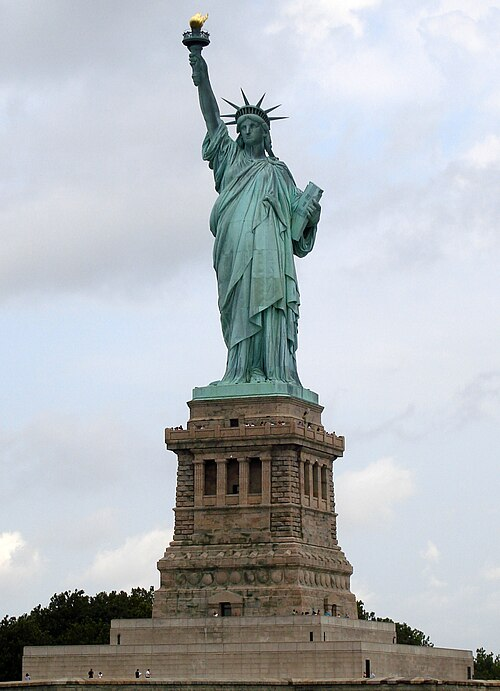
\includegraphics[width=0.32\linewidth]{images/book3/liberty.jpg}

{\small Sebuah patung tembaga yang berusia lebih dari satu abad: kulitnya
yang berupa lembaran tembaga tipis telah menjadi hijau, tertutup patina
garam-garam basa tembaga yang melindungi logam di bawahnya. (Foto:
Elcobbola, domain publik, Wikimedia Commons.)}
\end{omfigure}

\section{Proteksi}

Korosi dilawan dengan memisahkan logam dari air dan oksigen (cat, plastik,
email, atau lapisan logam lain), dengan mengubah mediumnya (menghilangkan
oksigen, menambahkan inhibitor yang teradsorpsi pada logam), atau dengan
menggeser potensial logam ke dalam daerah imunitasnya.

\begin{definition}[Proteksi katodik]\label{def:b2:corrosion:protection}
Yang disebut \emph{proteksi katodik}\index{proteksi katodik} adalah
penurunan potensial sebuah struktur logam sampai oksidasinya berhenti,
dengan menjadikannya katode sebuah sel. Sel itu dapat dibentuk dengan
\emph{anode korban}\index{anode korban}, yaitu logam yang kurang mulia
(seng, magnesium, paduan aluminium) yang dihubungkan dengan struktur itu
dan habis terpakai menggantikannya, atau digerakkan oleh generator, dalam
\emph{proteksi arus paksa}\index{proteksi arus paksa}, dengan anode berupa
elektrode inert yang ditanam di dekatnya.
\end{definition}

\begin{proposition}[Umur anode korban]\label{prop:b2:corrosion:anode-life}
\omterm{def:b2:corrosion:protection}{Anode korban} bermassa $m$ dan bermassa molar $M$, yang dioksidasi dengan $n$
elektron dan efisiensi $\eta$ (fraksi logam yang menghasilkan arus berguna,
sisanya terkorosi dengan sendirinya), memberikan arus $I$ selama waktu
\[
  t = \frac{\eta\,m\,nF}{M I} .
\]
\end{proposition}

\begin{proof}
Muatan bergunanya adalah $\eta\,(m/M)\,nF$; bagilah dengan arusnya.
\end{proof}

\begin{omfigure}
\begin{tikzpicture}[font=\small, >={Stealth}]
  \fill[brown!20] (-4.2,-2.4) rectangle (4.2,0);
  \draw[thick] (-4.2,0) -- (4.2,0);
  \node[font=\scriptsize, anchor=south west] at (-4.2,0) {tanah};
  \fill[black!40] (-3.5,-1.6) rectangle (3.5,-1.2);
  \node[font=\scriptsize, white] at (0,-1.4) {pipa baja (katode)};
  % sacrificial anode
  \fill[black!65] (-3.2,-2.3) rectangle (-2.2,-1.95);
  \node[font=\scriptsize, anchor=north] at (-2.7,-2.3) {anode Mg};
  \draw[thick] (-2.7,-1.95) -- (-2.7,-1.6);
  \draw[->, omProp, thick] (-2.2,-2.12) -- (-1.4,-1.7);
  \node[font=\scriptsize, omProp, anchor=west] at (-1.9,-2.2) {arus di dalam tanah};
  % impressed current
  \draw[thick, rounded corners] (1.8,0.4) rectangle (3.2,1.2);
  \node[font=\scriptsize] at (2.5,0.8) {penyearah};
  \fill[black!65] (3.4,-2.3) rectangle (3.9,-1.8);
  \node[font=\scriptsize, anchor=north] at (3.65,-2.3) {anode inert};
  \draw[thick] (3.2,0.8) -- (3.65,0.8) -- (3.65,-1.8);
  \draw[thick] (1.8,0.8) -- (1.2,0.8) -- (1.2,-1.2);
  \node[font=\scriptsize, anchor=south] at (3.65,0.85) {$+$};
  \node[font=\scriptsize, anchor=south] at (1.2,0.85) {$-$};
  \node[font=\scriptsize, align=center] at (-2.7,0.8) {anode korban};
  \node[font=\scriptsize, align=center] at (2.5,1.55) {arus paksa};
\end{tikzpicture}

{\small \omterm{def:b2:corrosion:protection}{Proteksi katodik} pipa yang ditanam, skematis. Kiri: anode magnesium,
yang dihubungkan dengan kabel ke pipa, terkorosi menggantikannya. Kanan:
penyearah mengalirkan arus dari anode inert melalui tanah ke dalam pipa.}
\end{omfigure}

\begin{omfigure}
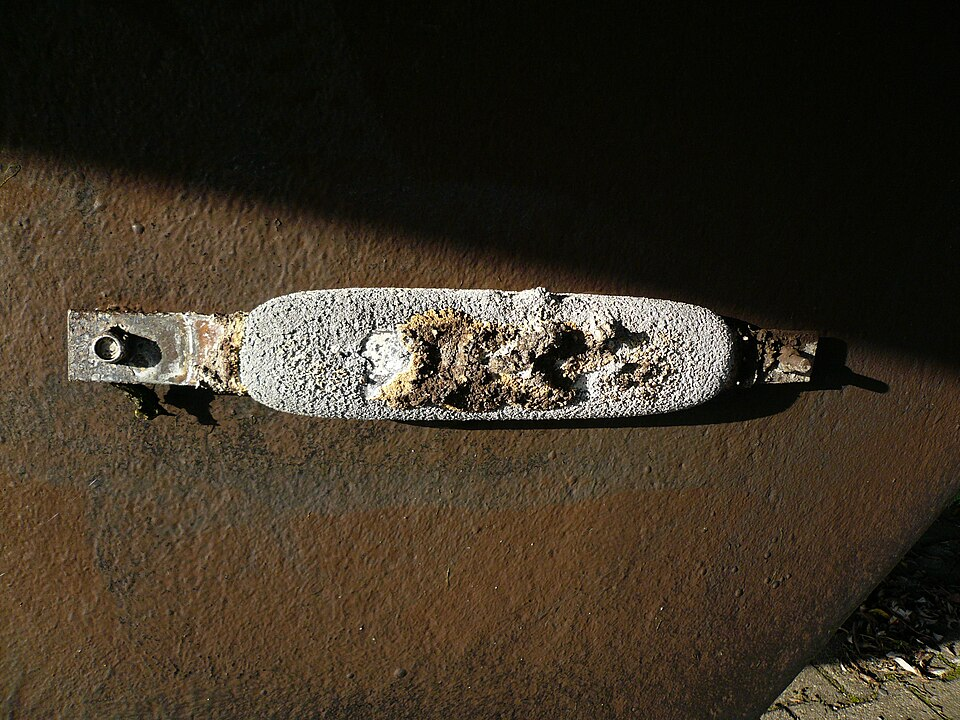
\includegraphics[width=0.5\linewidth]{images/book3/sacrificial-anode.jpg}

{\small \omterm{def:b2:corrosion:protection}{Anode korban} dari seng yang dibaut pada lambung baja sebuah kapal,
setelah satu musim di dalam air: sengnya habis termakan, baja di
sekelilingnya utuh. (Foto: Zwergelstern, CC BY-SA 3.0, Wikimedia
Commons.)}
\end{omfigure}

\begin{omfigure}
\begin{tikzpicture}[font=\small, >={Stealth}, scale=1.35]
  \begin{scope}
    \fill[black!25] (0,0) rectangle (4,0.6);
    \fill[gray!55] (0,0.6) rectangle (1.7,0.8); \fill[gray!55] (2.3,0.6) rectangle (4,0.8);
    \fill[omDef!15] (0.8,0.8) .. controls (1.3,1.3) and (2.7,1.3) .. (3.2,0.8) -- (2.3,0.8) -- (2.3,0.6) -- (1.7,0.6) -- (1.7,0.8) -- cycle;
    \node[font=\scriptsize] at (2,-0.3) {baja galvanis (lapisan seng)};
    \node[font=\scriptsize, align=center] at (2,1.6) {seng terkorosi,\\ baja terlindungi};
    \draw[->, omThm] (1.4,0.85) -- (1.8,0.65);
  \end{scope}
  \begin{scope}[xshift=5.5cm]
    \fill[black!25] (0,0) rectangle (4,0.6);
    \fill[gray!25] (0,0.6) rectangle (1.7,0.8); \fill[gray!25] (2.3,0.6) rectangle (4,0.8);
    \fill[omDef!15] (0.8,0.8) .. controls (1.3,1.3) and (2.7,1.3) .. (3.2,0.8) -- (2.3,0.8) -- (2.3,0.6) -- (1.7,0.6) -- (1.7,0.8) -- cycle;
    \fill[omProp] (1.75,0.6) rectangle (2.25,0.45);
    \node[font=\scriptsize] at (2,-0.3) {baja berlapis timah (lapisan timah)};
    \node[font=\scriptsize, align=center] at (2,1.6) {baja terkorosi di goresan,\\ cepat (anode kecil)};
  \end{scope}
\end{tikzpicture}

{\small Goresan yang menembus lapisan logam, skematis. Seng, yang kurang
mulia daripada besi, menjadi anode dan melindungi baja yang terbuka, berapa
pun ukuran goresannya. Timah, yang lebih mulia daripada besi, menjadi
katode besar di sekeliling anode baja yang kecil, yang terkorosi lebih
cepat daripada baja telanjang.}
\end{omfigure}

\begin{method}[Memilih proteksi]\label{met:b2:corrosion:choose-protection}
\begin{enumerate}
  \item Hindari pasangan galvanik: isolasi logam-logam yang berbeda, atau
        jadikan logam yang kurang mulia sebagai yang lebih luas.
  \item Lapisi: lapisan penghalang (cat, timah) hanya melindungi selama
        utuh; lapisan korban (seng) tetap melindungi walaupun tergores.
  \item Untuk struktur di dalam tanah atau air laut, tambahkan \omterm{def:b2:corrosion:protection}{proteksi
        katodik}: \omterm{def:b2:corrosion:protection}{anode korban} untuk arus kecil atau air yang konduktif, arus
        paksa untuk struktur panjang atau tanah yang resistif.
  \item Jangan memproteksi berlebihan: potensial yang terlalu rendah
        mereduksi air menjadi hidrogen pada struktur, yang mengelupas
        lapisan pelindung dan dapat membuat baja berkekuatan tinggi
        menjadi rapuh.
\end{enumerate}
\end{method}

\section{Latihan}

\begin{exercise}[$\star$]\label{exo:b2:corrosion:1}
Seng terkorosi secara seragam di bawah rapat arus \qty{2.0}{\micro A/cm^2}.
Hitunglah kehilangan ketebalannya per tahun ($\rho = \qty{7.13}{g/cm^3}$).
\end{exercise}

\begin{exercise}[$\star$]\label{exo:b2:corrosion:2}
Baut-baut baja memegang lembaran-lembaran tembaga pada sebuah atap. Logam
mana yang terkorosi? Pertanyaan yang sama untuk paku seng pada lembaran
baja.
\end{exercise}

\begin{exercise}[$\star$]\label{exo:b2:corrosion:3}
Dua pelat baja disatukan oleh sebuah baut dan dibiarkan di dalam air laut.
Di mana korosi terpusat, dan mengapa?
\end{exercise}

\begin{exercise}[$\star$]\label{exo:b2:corrosion:4}
Sebuah ember galvanis dan sebuah kaleng timah sama-sama tergores sampai ke
bajanya. Mana yang berkarat di goresannya?
\end{exercise}

\begin{exercise}[$\star\star$]\label{exo:b2:corrosion:5}
Pada diagram Evans besi dalam air beraerasi, jelaskan apa yang terjadi pada
potensial dan \omterm{def:b2:corrosion:uniform}{arus korosi} ketika air diaduk, lalu ketika air dibebaskan
dari oksigen.
\end{exercise}

\begin{exercise}[$\star\star$]\label{exo:b2:corrosion:6}
Sebuah anode seng \qty{5.0}{kg} melindungi lambung kapal dengan arus
\qty{0.10}{A}, dengan efisiensi 90~\% (data latihan). Berapa lama anode itu
bertahan?
\end{exercise}

\begin{exercise}[$\star\star$]\label{exo:b2:corrosion:7}
Hitunglah muatan, dalam ampere-jam per kilogram, yang diberikan oleh anode
seng, magnesium, dan aluminium pada efisiensi 100~\%, serta potensial
standar pasangan-pasangannya dari $\Delta_f G^\circ$ (\ce{Zn^2+} $-147.06$,
\ce{Mg^2+} $-454.8$, \ce{Al^3+} $-485$ \unit{kJ/mol}). Mengapa magnesium
lebih disukai di tanah kering?
\end{exercise}

\begin{exercise}[$\star\star$]\label{exo:b2:corrosion:8}
Sebuah pipa yang ditanam memerlukan arus proteksi \qty{2.0}{A}. Hamparan
anode inert mempunyai hambatan \qty{4.0}{\ohm} terhadap tanah, dan selnya
memerlukan tambahan \qty{1.5}{V} (data latihan). Hitunglah tegangan
penyearah dan energi listrik per tahun.
\end{exercise}

\begin{exercise}[$\star\star$]\label{exo:b2:corrosion:9}
Sebuah tiang pancang baja berdiri di laut. Jelaskan mengapa tiang itu
paling banyak terkorosi sedikit di bawah garis air, dan tidak tepat di
garis air.
\end{exercise}

\begin{exercise}[$\star\star\star$]\label{exo:b2:corrosion:10}
Jelaskan, dengan kurva pasif, mengapa baja tahan karat tahan terhadap air
beraerasi tetapi dapat mengalami sumuran di air laut, dan mengapa sebuah
sumuran, begitu terbentuk, tumbuh makin dalam alih-alih makin lebar.
\end{exercise}

\begin{exercise}[$\star\star\star$]\label{exo:b2:corrosion:11}
Sebuah sambungan tembaga disekrupkan pada pipa baja yang mengalirkan air
beraerasi. Rapat \omterm{def:b2:current-potential-curves:limiting-current}{arus pembatas} oksigen adalah \qty{5}{\micro A/cm^2} pada
setiap permukaan yang basah; tembaga menyediakan \qty{20}{cm^2} dan baja di
dekat sambungan \qty{2}{cm^2} (data latihan). Perkirakan \omterm{def:b2:corrosion:uniform}{arus korosi} baja
dan kehilangan ketebalannya per tahun di dekat sambungan.
\end{exercise}

\begin{exercise}[$\star\star\star$]\label{exo:b2:corrosion:12}
Dengan diagram E--pH besi dan kurva-kurva air, jelaskan mengapa potensial
struktur baja yang diproteksi harus dijaga di bawah sekitar \qty{-0.6}{V}
tetapi tidak jauh di bawah \qty{-1}{V} dalam air netral.
\end{exercise}

\section{Soal: Memproteksi Sebuah Pipa Saluran}

\begin{problem}[{Soal akhir pekan --- korosi pipa baja telanjang di dalam
tanah basah, pemilihan logam korban, magnesium yang diperlukan untuk dua
puluh tahun, dan alternatif arus paksa}]
\label{pb:b2:corrosion:1}
Sebuah pipa saluran baja sepanjang \qty{10.0}{km} dengan diameter
\qty{0.30}{m} ditanam di dalam tanah basah. Data: besi
$M = \qty{55.845}{g/mol}$, $\rho = \qty{7.87}{g/cm^3}$; magnesium
$M = \qty{24.305}{g/mol}$; $\Delta_f G^\circ$ (\unit{kJ/mol}): \ce{Fe^2+}
$-78.90$, \ce{Zn^2+} $-147.06$, \ce{Mg^2+} $-454.8$, \ce{Al^3+} $-485$. Data
latihan: rapat \omterm{def:b2:corrosion:uniform}{arus korosi} baja telanjang di tanah ini \qty{10}{\micro
A/cm^2}; rapat arus rancangan untuk proteksi baja telanjang
\qty{20}{mA/m^2}; lapisan pelindungnya menyisakan 1.0~\% permukaan yang
telanjang; anode magnesium \qty{15}{kg}, efisiensi 50~\%; hambatan hamparan
anode untuk arus paksa \qty{5.0}{\ohm}.
% ledger: aw:Fe, rho:Fe, aw:Mg, dfg:Fe2+_ao, dfg:Zn2+_ao, dfg:Mg2+_ao, dfg:Al3+_ao, const:F

\medskip
\noindent\textbf{Bagian I --- Pipa telanjang.}
\begin{enumerate}
  \item Tuliskan reaksi anodik dan reaksi katodik pada pipa itu.
  \item Mengapa \omterm{def:b2:corrosion:uniform}{arus korosi} ditetapkan oleh pasokan oksigen?
  \item Hitunglah massa besi yang hilang per meter persegi per tahun.
  \item Hitunglah kehilangan ketebalan dinding per tahun.
  \item Berapa lama pipa telanjang itu akan kehilangan separuh dari dinding
        setebal \qty{8}{mm}?
  \item Mengapa pipa yang sebenarnya rusak lebih cepat, pada beberapa
        titik?
\end{enumerate}

\medskip
\noindent\textbf{Bagian II --- Logam anode.}
\begin{enumerate}[resume]
  \item Hitunglah potensial standar pasangan-pasangan besi, seng,
        magnesium, dan aluminium.
  \item Logam-logam mana yang dapat melindungi besi sebagai \omterm{def:b2:corrosion:protection}{anode korban}?
  \item Mengapa aluminium jarang dipakai di dalam tanah?
  \item Mengapa magnesium lebih disukai daripada seng di tanah yang
        resistivitasnya tinggi?
  \item Hitunglah massa magnesium yang terpakai per ampere per tahun.
\end{enumerate}

\medskip
\noindent\textbf{Bagian III --- Rancangan.}
\begin{enumerate}[resume]
  \item Hitunglah luas permukaan luar pipa.
  \item Hitunglah luas permukaan telanjang yang ditinggalkan lapisan
        pelindung.
  \item Hitunglah arus proteksinya.
  \item Hitunglah muatan yang diperlukan untuk dua puluh tahun.
  \item Hitunglah massa magnesium yang diperlukan.
  \item Berapa anode yang diperlukan?
  \item Mengapa anode-anode itu disebar di sepanjang pipa alih-alih ditanam
        di satu titik?
\end{enumerate}

\medskip
\noindent\textbf{Bagian IV --- Arus paksa.}
\begin{enumerate}[resume]
  \item Uraikan alternatif arus paksa.
  \item Perkirakan tegangan penyearah dari hambatan hamparan anode, dengan
        menambahkan \qty{1.5}{V} untuk elektrode-elektrodenya.
  \item Hitunglah energi listrik yang dipakai per tahun.
  \item Apa yang salah jika pipa itu diproteksi berlebihan?
  \item Di bawah potensial berapa besi imun dalam air netral, dengan
        menganggap konsentrasi besi(II) \qty{1e-6}{mol/L}?
  \item Nyatakan massa anode magnesium yang diperlukan untuk dua puluh
        tahun.
\end{enumerate}
\end{problem}
